\chapter{Background}
\label{chap:background}
%----------------------------------------------------------------------------------------
This chapter provides an overview of the main concepts and technologies on which it is based this thesis. \Cref{sec:AC} introduces the Aggregate Computing paradigm; it discusses its core idea, the theory and basic functionalities under it, and finally presents Protelis, a language for this paradigm. 
Then, \Cref{sec:LoRaWAN} introduces the LoRaWAN network protocol. 
Finally, \Cref{sec:DingNet} introduces the DingNet LoRaWAN network and relative simulator. 

\section{Aggregate Computing}
\label{sec:AC}
Recent technological developments led to computational and networking capabilities being more and more integrated with everyday objects. 
% 
Not only personal smartphone but also the all set of wearable device, drones, smart vehicular system, domestic appliances and more generally all kind of sensor and actuator.
% 
This development led to design distributed system with always more and different devices (mainly for computational capability and communication technology) producing pervasive heterogeneous and complex system.
% 
The classic approach for distributed system proposes a device-centric viewpoint.
% 
The goal is to obtain global behaviour as emergent phenomena from the interaction of single devices. 
% 
So the focus of the designer is on local structure, behaviour, and interaction. 
% 
The final result is typically a system strongly dependent on communication technology that tends to be rigid and costly to testing, evolve, and maintain.
 
Aggregate computing is an emerging programming paradigm devoted to modern distributed systems~\cite{BealIEEEComputer2015}, which proposes a shift of paradigm and viewpoint respect the problem. 
% 
It proposes an aggregate viewpoint where the programmable entity is the entire set of devices.
% 
The goal is to define the global behaviour in a declarative way focusing on manipulation of spatial and temporal data structures. This allows the designer to abstract from the real device that will execute the program, its communication capability, network infrastructure, and its execution platform~\cite{ViroliUbiComp2016}. 
% 
The final result will be a complex, modular, extendible, self-adaptive and self-organized distributed system.
% 
The aggregate computing approach offers base functionalities that are combinable with each other to assemble advanced and user-friendly APIs. In order to organize all the provided functionalities, a multilayer stack has been designed, which collects them all by abstraction level. 
As is possible seeing from the stack, \autoref{fig:ACstack}, the base constructs are based on the \textit{field calculus} theory.

\begin{figure}[h]
    \centering
    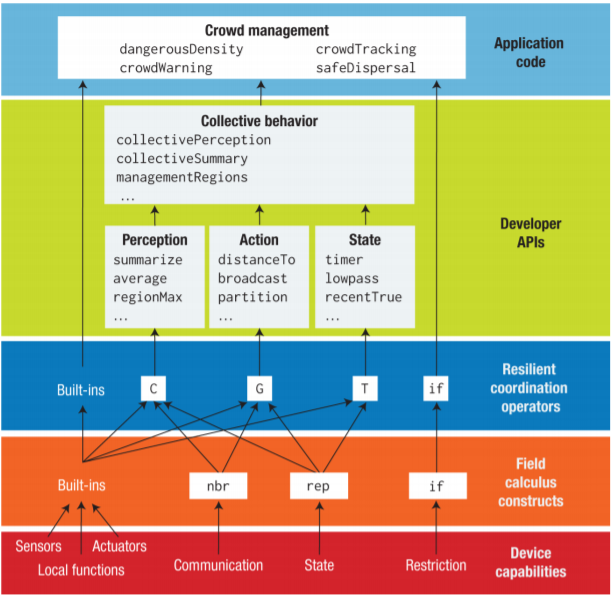
\includegraphics{figures/ACstack.png}
    \caption[Aggregate programming stack]{Aggregate programming stack.~\cite{BealIEEEComputer2015}}
    \label{fig:ACstack}
\end{figure}

\subsection{Field-calculus}

Field calculus is a theoretical model that describes a set of primitives to manipulate the concept of \textit{computational field}. A computational field is a distributed data structure that maps every networked device to some local value. In field calculus, everything is a field (value, variable, expression, function) and the constructs to build and manipulate it are:
\begin{itemize}
    \item \textbf{Functions}, $b(e1,\dots,e_n)$ applies function $b$ to arguments $e1,\dots,e_n$. The output field is obtained by the point-wise evaluation of the operator to the input fields
    \item \textbf{Stateful computation}, $rep(x \leftarrow v)~\{s1; \dots ; s_n\}$ a local variable $x$ is defined and initialized to value $v$. Then the value is periodically updated with the result of statements $s1; \dots ; s_n$
    \item \textbf{Interaction}, $nbr(s)$ share the local value of $s$, represented as a field, with its neighbours. The result is a field of fields (the same information shared from neighbours) that is possible to reduce to a simple field using \textit{hood} operators
    \item \textbf{Domain restriction}, $if(e)~\{s1; \dots ; s_n\}~else~\{s'_1; \dots ; s'_n\}$ split the field in two sub-field according to the evaluation of $e$. Where $e$ is true is applied the statement $s1; \dots ; s_n$, while where $e$ is false is applied the statement $s'_1; \dots ; s'_n$.
\end{itemize}

The behaviour of aggregate systems can be expressed as a functional composition of operators that manipulate (evolve, combine, restrict) computational fields~\cite{type-sound}.

\subsection{Building blocks operators}
Basic field calculus constructors are low-level operators and led to error-prone programming. In order to limit the use of these  operators,~\cite{buildingBlock} present the set of building block that compose the central layer of the aggregate programming stack, \autoref{fig:ACstack}. These functionalities are then available as library function defined on top of the low-level operators. The principal functions presented are:

\begin{itemize}
    \item $G(source, init, metric, accumulate) \rightarrow$ function to spreading information across space. First, build a field of the shortest path that starts from the $source$ with the chosen $metric$. Then spread the information across the field starting from the $init$ value and modifying it at each step with the $accumulate$ function
    \item $C(potential, reduce, local, null) \rightarrow$ function to accumulates $local$ value along the $potential$ field until the source. The final value is obtained applying the $reduce$ function to the $local$ value of the crossed nodes. If there is nothing to accumulate is returned the default value $null$
    \item $T(init, zero, decay)  \rightarrow$ function to evolve the state for a specified period. The period start from $init$ and decrease until $zero$ with a $decay$ rate
    \item $S(grain, metric)  \rightarrow$ function to split the network into partitions of nodes. This function uses the $metric$ function to define the sets of nodes of size $grain$ and elects a leader for each partition.
\end{itemize}

Reduce the possibility to make mistake with low-level operators is not the only advantage in using this building block.
This functions are also complementary and combining them differently is possible to implement all the principal coordination patterns for distributed system. Finally, another advantage is that these functions are self-stabilizing and consequently systems build on top of them will be self-stabilizing. In complex system, self-stabilizing property guarantee that after each transitory phase, the system return to a stationary state (if exists), where it is possible to predict its behaviour.


\subsection{Protelis}
\label{subSec:Protelis}
Protelis~\cite{PianiniSAC2015} is a language designed for the ``aggregate computing" paradigm built on field calculus and inspired on Proto~\cite{Proto}. 
It offers an implementation of the entire aggregate computing stack, and support for high-order field calculus~\cite{ViroliTOCL2016}, that introduces functions as first-class citizen with a lot of benefits.
Protelis adopts a C- or Java-like syntax to reduce learning care, but it is a pure functional language.
Aggregate computing is a paradigm for heterogeneous distributed system, and one important requirement for languages for this paradigm is interoperability.
Protelis absolves it because it is executed on the Java Virtual Machine%that guarantee interoperability
, but this means also full interoperability with Java world and access to all the plethora of its library.
Accordingly to aggregate programming principles a Protelis program abstract from implementation of device capabilities, real network topology and technology. 
To fill this abstraction gap Protelis requires to implement a back-end for every node of the system.
It requires the implementation of two interfaces \textit{ExecutionContext} and \textit{NetworkManager}. 
The first represents the context of the node (similar to \textit{System} or \textit{Runtime} in Java) and requires the implementation of some function. It is also the entry point for specific device capabilities and spatio-temporal information on the node. The second one requires the implementation of two methods to enable the communication with the other nodes, filling the abstraction gap between real and logical network.
\clearpage
\section{LoRaWAN}
\label{sec:LoRaWAN}

In the context of smart-city and more generally of the Internet of Things (IoT) one important requirement is to reduce the ``things'' cost, intended as cost to buy it, and for its maintenance without compromise the communication range.
Low-power wide-area network~\cite{Raza2017} (LPWAN) is a type of wireless network to allow long-range communication requiring low power consumption.
Typically devices for this type of networks have communication range from few kilometers in urban areas to over 10 Km in open-space areas.
Low cost requirement is achieve as composition of three factor:
\begin{itemize}
    \item use of lightweight protocols $\rightarrow$ this means device with simple hardware, so cheaper device
    \item use of licence-free or licensed band $\rightarrow$ this means reduction of network cost
    \item low power communication $\rightarrow$ this allows run device with small battery for over 10 years reducing cost for maintenance.
\end{itemize}

LoRaWAN~\cite{loraalliancetechnicalcommittee2020} is one of the main LPWAN protocol.
A LoRaWAN network, \autoref{fig:LoRaNetwork}, is composed of three fundamental elements: end-device (aka motes), gateway (aka concentrators) and a network-server. 
% 
The topology of the network typically is a star-of-stars topology with the gateway that intermediate between motes and network-server.
% 
The communication between gateway and network-server is IP-based, while the communication between gateway and motes uses the LoRa (Long Range) modulation.

\begin{figure}[h]
    \centering
    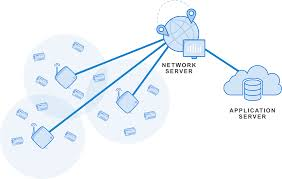
\includegraphics{figures/lora_architecture2.png}
    \caption[LoRaWAN network architecture]{LoRaWAN network architecture~\cite{muntasirjoarder2020} with all the fundamental elements. Straight lines represent IP-based communication, while the circle around the gateways is the communication range based on LoRa modulation.}
    \label{fig:LoRaNetwork}
\end{figure}

The role of network-server is to govern and optimize the interactions between motes and gateways and provides the mote's packet to applications in the application server.
% 
So among other tasks, it has to filter duplicated packet received from gateways and find the best gateway to deliver an application message to a mote.
% 
The LoRaWAN protocol, \autoref{fig:LoRaStack}, is composed of two layers: the  physical layer and the MAC one.

\begin{figure}[h]
    \centering
    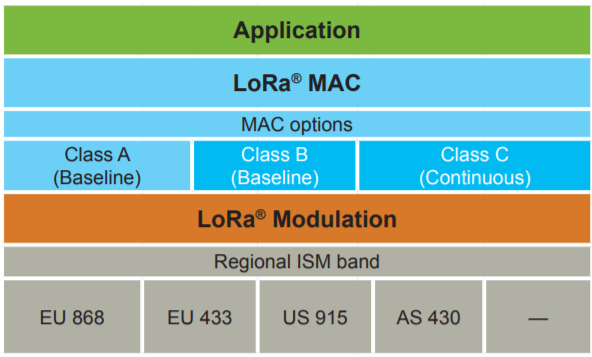
\includegraphics{figures/loraStack.png}
    \caption[LoRaWAN protocol stack]{LoRaWAN protocol stack~\cite{loraalliance2020} where brown rectangle represent the physical layer and the azures rectangles the MAC one.}
    \label{fig:LoRaStack}
\end{figure}

\subsection{Physical Layer}
The physical layer implements the LoRa protocol allowing communication until 15 Km of distance, with a data rate from 0.3 Kb/s to 11 Kb/s with LoRa modulation, and to 50 kb/s with FSK modulation.
% 
The most important parameters for LoRa modulation are Bandwidth (BW), Spreading Factor (SF) and the Code Rate (CR).
% 
The SF value is in the range from 7 to 12 and represents the number of bits in each symbol.
% 
It is an important parameter because define: the maximum packet length, the range of communication and the bit rate.
% 
SF7 means longest packet length and highest bit rate, but shortest communication range; while SF12 means shortest packet length and lowest bit rate, but longest communication range.
% 
Another important aspect of SF is that concurrent transmission with different SF will not produce any collision between the two transmissions.
% 
Finally, LoRa uses the regional Industrial, Scientific and Medical (ISM) band. This means lower network cost, but limitation of the duty \mbox{cycle} to maximum 1\% for each channel imposed from the European telecommunications standards institute (ETSI).

\subsection{MAC Layer}
% (Class A, B and C)
The aim of this layer is to regulate communications between motes and gateways.
% 
Uplink communication (mote to gateways) uses an ALOHA-like protocol. Motes start a broadcast communication when they need without checking channel's state, but applying a small random delay.
% 
For downlink communication (gateway to mote) to reduce the battery consumption of the motes, and respect latency requirement of different applications, the MAC layer defines three different classes of devices (A, B and C) with different behaviour.
% 
Devices of class A define two fixed receiving windows after each uplink communication, with the second one opened only if the mote receives a communication during the first. 
% 
This class has the lowest battery consumption with the drawback of the highest latency. 
% 
Devices of class B allow to define more receive windows, but it is necessary to keep motes and server synchronized via synchronized Beacon. 
% 
This class has lower latency than class A but also higher battery consumption. 
% 
Finally, devices of class C allow always to receive messages except when they execute an uplink communication. 
% 
This class has the lowest latency, but the highest battery consumption.

\section{DingNet: a LoRa-over-MQTT network and simulator}
\label{sec:DingNet}
The LoRaWAN protocol does not standardize communications after the gateways, but defines only that are IP-based.
% 
LoRa-over-MQTT identifies a network where the communication between gateways and network-server is implemented using the public-subscribe pattern via MQTT protocol, and the application server provides data to applications in different ways, but at least via MQTT.
% 
An example of LoRa-over-MQTT architecture is ChirpStack\footnote{\href{https://www.chirpstack.io/}{https://www.chirpstack.io/} (Jan 2020)}, see \autoref{fig:ChirpStack}, that is an open-source LoRaWAN Network Server stack to manage all the LoRaWAN network components and provides data to applications in different ways.

\begin{figure}[h]
    \centering
    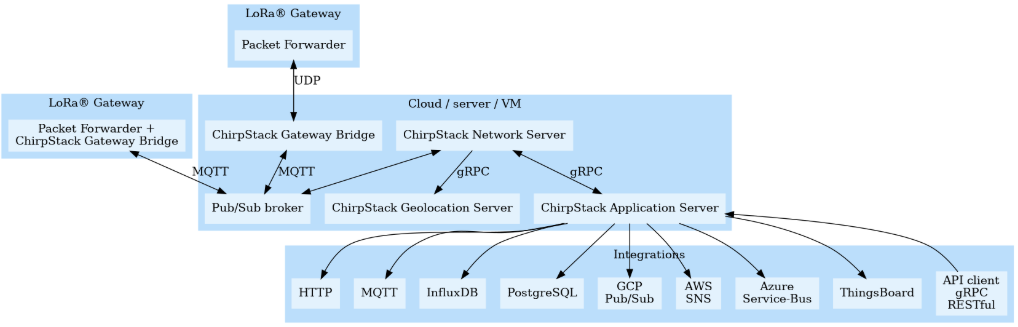
\includegraphics[width=\textwidth]{figures/chirpstack.png}
    \caption[LoRa-over-MQTT architecture]{Example of the LoRa-over-MQTT architecture of ChirpStack.~\cite{chirpstack2020}}
    \label{fig:ChirpStack}
\end{figure}

DingNet\footnote{\href{https://admin.kuleuven.be/icts/english/services/dingnet}{https://admin.kuleuven.be/icts/english/services/dingnet} (Jan 2020)} is a real LoRaWAN network of class A composed of 11 gateways that cover the entire university city of Leuven and adopts a LoRa-over-MQTT architecture. 
% 
DingNet allows adding user's devices and applications to the network for research porpoise.
% 
Last year was introduced the DingNet Simulator~\cite{inproceedings}.
It allows simulation of applications in different scenarios before deploying them in the real network to reduce costs and time for the deploy.
% 
It is a time-driven simulator focused on the simulation of LoRa communications between gateways and motes while the rest of the network is simulated with a higher-level of abstraction. 
% 
The simulator allows configuring the environment of the network in terms of position of gateways, motes, and typology of areas that compose the environment. 
% 
Exist different types of areas (like forest, open space, building area) to represent different kinds of areas present in a city. 
Each area differs for how much decrease the power of a transmission; for example, a building area decreases power more than an open space one.
% 
Motes can be stationary, but also mobile.
% 
For each mote is possible to configure all the most important parameters for a LoRa transmission, like bandwidth, spreading-factor and transmission power. 
% 
The simulator for each transmission computes the time-on-air based on the previous parameters and the size of the packet. 
% 
Then it applies an algorithm to decrease the power of transmission based on the distance from source and typology of areas that the transmission is going through to find all the gateway inside the communication range.
% 
Every transmission is considered arrived at a gateway when is pass enough time (time-on-air) from the beginning of the transmission. 
Finally, the gateway applies a particular algorithm to check if the transmission is collided with others. If not it publishes the received packet on an MQTT broker for the applications.
%
At the end of each simulation is possible to export different information for mote's transmission:
\begin{itemize}
    \item received power from the gateways (dBm)
    \item time on air (ms)
    \item used power for the transmission (dBm)
    \item used energy for the transmission (mJoule)
    \item collision with others transmissions (true/false).
\end{itemize}

Nowadays, the simulator is used mainly to simulate self-adaptive applications in large scenarios to increase the number of transmissions correctly delivered to at least one gateway reducing the energy consumption of the motes.

\paragraph{Concluding} this chapter has presented first the aggregate computing paradigm, presenting its benefits for pervasive and heterogeneous systems, and the language Protelis. Then it had presented LoRaWAN, which is one of the main LPWAN protocol. 
Finally it has presented DingNet a LoRaWAN network and its simulator.